% ============================================================
\chapter{Network Flows}
\label{ch:flows}
% ============================================================

\section{Introduction}

In 1956, at the height of the Cold War, mathematicians Lester Ford and Delbert Fulkerson at the RAND Corporation worked on a strategic problem: what is the maximum capacity of the Soviet railway network between the USSR and Eastern Europe? To answer this, they developed the Ford--Fulkerson algorithm and proved the max-flow min-cut theorem, one of the most elegant results in combinatorial optimization: the maximum flow from a source to a sink equals exactly the minimum capacity of any cut separating them. This profound duality between flows and cuts now irrigates logistics, telecommunications, computer vision, and even bioinformatics.

\begin{intuition}
Imagine a network of pipes connecting a water source to a reservoir. Each pipe
has a maximum capacity. The maximum flow problem asks for the greatest rate at
which water can be shipped from source to reservoir while respecting every
pipe's capacity.
\end{intuition}

\section{Fundamental definitions}

\begin{definition}[Flow network]
\index{flow network}
A \textbf{flow network} is a directed graph $G = (V, A)$ equipped with a
capacity function $c : A \to \R_+$, a \textbf{source} vertex $s \in V$, and a
\textbf{sink} vertex $t \in V$ with $s \ne t$.
\end{definition}

\begin{definition}[Flow]
\index{flow}
A \textbf{flow} in a network $(G, c, s, t)$ is a function $f : A \to \R_+$
satisfying:
\begin{enumerate}
  \item \textbf{Capacity constraint}: $0 \leq f(u,v) \leq c(u,v)$ for all
        $(u,v) \in A$.
  \item \textbf{Flow conservation}: for every $v \in V \setminus \{s, t\}$,
        \[
          \sum_{u : (u,v) \in A} f(u,v) = \sum_{w : (v,w) \in A} f(v,w).
        \]
\end{enumerate}
The \textbf{value} of the flow is $\abs{f} = \sum_{w : (s,w) \in A} f(s,w)
- \sum_{u : (u,s) \in A} f(u,s)$.
\end{definition}

\begin{definition}[Residual graph]
\index{residual graph}
Given a flow $f$, the \textbf{residual graph} $G_f = (V, A_f)$ is defined by:
\begin{itemize}
  \item For each arc $(u,v) \in A$ with $f(u,v) < c(u,v)$: forward arc
        $(u,v)$ with residual capacity $c_f(u,v) = c(u,v) - f(u,v)$.
  \item For each arc $(u,v) \in A$ with $f(u,v) > 0$: backward arc $(v,u)$
        with residual capacity $c_f(v,u) = f(u,v)$.
\end{itemize}
\end{definition}

\begin{definition}[Augmenting path]
\index{augmenting path}
An \textbf{augmenting path} is a path from $s$ to $t$ in the residual graph
$G_f$. Its \textbf{bottleneck capacity} is the minimum residual capacity
along the path.
\end{definition}

\begin{definition}[Cut]
\index{cut}
A \textbf{cut} $(S, T)$ is a partition of $V$ into $S$ and $T = V \setminus S$
with $s \in S$ and $t \in T$. Its \textbf{capacity} is:
\[
  c(S, T) = \sum_{\substack{u \in S,\, v \in T \\ (u,v) \in A}} c(u,v).
\]
\end{definition}

\section{Max-flow min-cut theorem}

\begin{theorem}[Max-flow min-cut]
\label{thm:maxflow_mincut}
\index{max-flow min-cut theorem}
In any flow network, the maximum value of a flow equals the minimum capacity
of a cut:
\[
  \max_f \abs{f} = \min_{(S,T)} c(S, T).
\]
\end{theorem}

\begin{proof}
\textbf{Step 1} (weak duality): For any flow $f$ and any cut $(S, T)$:
\[
  \abs{f} = \sum_{\substack{u \in S,\, v \in T}} f(u,v)
          - \sum_{\substack{u \in T,\, v \in S}} f(u,v)
          \leq \sum_{\substack{u \in S,\, v \in T}} c(u,v) = c(S, T).
\]

\textbf{Step 2}: If $f$ has no augmenting path in $G_f$, define
$S = \{v \in V : v \text{ is reachable from } s \text{ in } G_f\}$ and
$T = V \setminus S$. Then $s \in S$ and $t \in T$.

\textbf{Step 3}: For every arc $(u,v)$ with $u \in S, v \in T$, we have
$f(u,v) = c(u,v)$ (otherwise $(u,v) \in A_f$ and $v$ would be in $S$).
For every arc $(v,u)$ with $v \in T, u \in S$, $f(v,u) = 0$. Hence
$\abs{f} = c(S, T)$.
\end{proof}

\begin{keyformulas}[title=\textbf{Key flow properties}]
\begin{itemize}
  \item $\abs{f} \leq c(S,T)$ for every cut $(S,T)$.
  \item A flow is maximum $\iff$ no augmenting path exists.
  \item $\max \abs{f} = \min c(S,T)$ (max-flow min-cut theorem).
  \item If capacities are integral, there exists an integral max flow.
\end{itemize}
\end{keyformulas}

\section{Ford-Fulkerson algorithm}

\begin{algorithme}[title=\textbf{Ford-Fulkerson}]
\index{Ford-Fulkerson algorithm}
\begin{enumerate}
  \item Initialize $f(u,v) = 0$ for all arcs.
  \item While there exists an augmenting path $P$ from $s$ to $t$ in $G_f$:
    \begin{enumerate}
      \item Compute $\delta = \min_{(u,v) \in P} c_f(u,v)$.
      \item For each arc $(u,v) \in P$: update flow along $P$ by $\delta$.
    \end{enumerate}
  \item Return $f$.
\end{enumerate}
\end{algorithme}

\begin{warning}[title=\textbf{Termination of Ford-Fulkerson}]
With irrational capacities, Ford-Fulkerson may not terminate. With integer
capacities, the complexity is $\mathcal{O}(\abs{A} \cdot \abs{f^*})$ where
$\abs{f^*}$ is the max flow value, which can be very large.
\end{warning}

\section{Edmonds-Karp algorithm}

\begin{theorem}[Edmonds-Karp]
\index{Edmonds-Karp algorithm}
The Edmonds-Karp algorithm is Ford-Fulkerson with BFS (shortest augmenting
path in terms of number of arcs). Its complexity is
$\mathcal{O}(\abs{V} \cdot \abs{A}^2)$.
\end{theorem}

\begin{proof}
One shows that the BFS distance from $s$ to any vertex $v$ in $G_f$ never
decreases across augmentations. Since each augmentation saturates at least one
\emph{critical} arc, and each arc can become critical at most $\abs{V}/2$
times, the total number of augmentations is $\mathcal{O}(\abs{V} \cdot
\abs{A})$. Each BFS costs $\mathcal{O}(\abs{A})$.
\end{proof}

\begin{example}[Maximum flow]
Consider the network with source $s$ and sink $t$:
\begin{center}
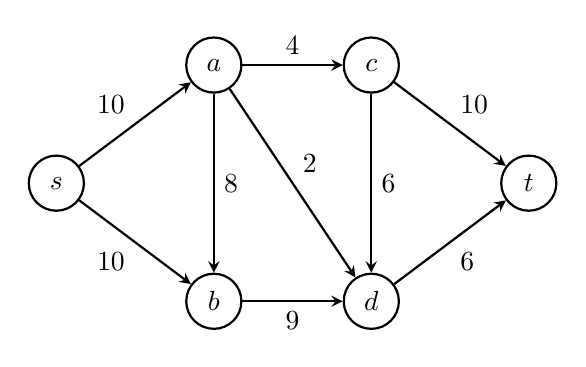
\begin{tikzpicture}[
    vertex/.style={circle, draw, minimum size=7mm, inner sep=0pt},
    >=stealth, thick
  ]
  \node[vertex] (s) at (0,1.5) {$s$};
  \node[vertex] (a) at (2,3) {$a$};
  \node[vertex] (b) at (2,0) {$b$};
  \node[vertex] (c) at (4,3) {$c$};
  \node[vertex] (d) at (4,0) {$d$};
  \node[vertex] (t) at (6,1.5) {$t$};
  \draw[->] (s) -- node[above left] {10} (a);
  \draw[->] (s) -- node[below left] {10} (b);
  \draw[->] (a) -- node[above] {4} (c);
  \draw[->] (a) -- node[right] {8} (b);
  \draw[->] (a) -- node[above right] {2} (d);
  \draw[->] (b) -- node[below] {9} (d);
  \draw[->] (c) -- node[above right] {10} (t);
  \draw[->] (d) -- node[below right] {6} (t);
  \draw[->] (c) -- node[right] {6} (d);
\end{tikzpicture}
\end{center}

Applying Edmonds-Karp yields a maximum flow of value 16.
\end{example}

\section{Minimum cost flows}

\begin{definition}[Minimum cost flow problem]
\index{minimum cost flow}
Given a network $G = (V, A)$ with capacities $c$, unit costs $w : A \to \R$,
and supply/demand $b : V \to \R$ with $\sum_{v} b(v) = 0$:
\[
  \min \sum_{(u,v) \in A} w(u,v) f(u,v) \quad \text{s.t.} \quad
  \begin{cases}
    0 \leq f(u,v) \leq c(u,v) & \forall (u,v) \in A, \\
    \displaystyle\sum_{u} f(u,v) - \sum_{w} f(v,w) = b(v)
    & \forall v \in V.
  \end{cases}
\]
\end{definition}

\begin{theorem}[Optimality condition]
A feasible flow $f$ has minimum cost if and only if there is no
\textbf{negative-cost cycle} in the residual graph $G_f$.
\end{theorem}

\section{Applications}

\subsection{Bipartite matching}

\begin{proposition}[Matching via max flow]
\index{bipartite matching}
The \textbf{maximum matching} in a bipartite graph $G = (U \cup W, E)$ reduces
to max flow: add source $s$ connected to all of $U$ and sink $t$ connected to
all of $W$, with all capacities equal to 1. The max flow value equals the
maximum matching size.
\end{proposition}

\begin{theorem}[K\"onig's theorem]
\index{K\"onig's theorem}
In a bipartite graph, the size of a maximum matching equals the size of a
minimum vertex cover.
\end{theorem}

\begin{proposition}[Menger's theorem]
\index{Menger's theorem}
The maximum number of edge-disjoint paths from $s$ to $t$ equals the minimum
number of edges whose removal disconnects $s$ from $t$.
\end{proposition}

\section{Python implementation}

\begin{codeblock}[title=\textbf{Edmonds-Karp implementation}]
\begin{minted}{python}
from collections import deque

def bfs(graph, s, t, parent):
    """BFS in the residual graph."""
    visited = {s}
    queue = deque([s])
    while queue:
        u = queue.popleft()
        for v in graph[u]:
            if v not in visited and graph[u][v] > 0:
                visited.add(v)
                parent[v] = u
                if v == t:
                    return True
                queue.append(v)
    return False

def edmonds_karp(graph, s, t):
    """Maximum flow via Edmonds-Karp."""
    max_flow = 0
    while True:
        parent = {}
        if not bfs(graph, s, t, parent):
            break
        delta = float('inf')
        v = t
        while v != s:
            u = parent[v]
            delta = min(delta, graph[u][v])
            v = u
        v = t
        while v != s:
            u = parent[v]
            graph[u][v] -= delta
            graph[v][u] += delta
            v = u
        max_flow += delta
    return max_flow
\end{minted}
\end{codeblock}

\section{Exercises}

\begin{exercise}[$\star$ -- Maximum flow]
Find the maximum flow in the network with $s$, $a$, $b$, $t$ and arcs
$s \to a$ (5), $s \to b$ (3), $a \to b$ (2), $a \to t$ (4), $b \to t$ (6).
Also find a minimum cut.
\end{exercise}

\begin{exercise}[$\star\star$ -- Edmonds-Karp trace]
Detail every iteration of Edmonds-Karp on the 6-vertex example network.
Show the residual graph at each step.
\end{exercise}

\begin{exercise}[$\star\star$ -- Bipartite matching]
Four employees $\{E_1, E_2, E_3, E_4\}$ can fill positions
$\{P_1, P_2, P_3, P_4\}$ with qualifications: $E_1$: $P_1, P_2$;
$E_2$: $P_2, P_3$; $E_3$: $P_1, P_3, P_4$; $E_4$: $P_3$.
Model as a flow problem and find a maximum matching.
\end{exercise}

\begin{exercise}[$\star\star\star$ -- Minimum cost flow]
A company ships goods from 2 factories to 3 warehouses. Formulate as a
minimum cost flow problem and solve.
\end{exercise}

\begin{exercise}[$\star\star\star$ -- Menger's theorem]
Show that Menger's theorem follows from max-flow min-cut. Apply to a
6-node telecommunications reliability problem.
\end{exercise}
